\documentclass[twoside]{book}

% Packages required by doxygen
\usepackage{fixltx2e}
\usepackage{calc}
\usepackage{doxygen}
\usepackage[export]{adjustbox} % also loads graphicx
\usepackage{graphicx}
\usepackage[utf8]{inputenc}
\usepackage{makeidx}
\usepackage{multicol}
\usepackage{multirow}
\PassOptionsToPackage{warn}{textcomp}
\usepackage{textcomp}
\usepackage[nointegrals]{wasysym}
\usepackage[table]{xcolor}

% Font selection
\usepackage[T1]{fontenc}
\usepackage[scaled=.90]{helvet}
\usepackage{courier}
\usepackage{amssymb}
\usepackage{sectsty}
\renewcommand{\familydefault}{\sfdefault}
\allsectionsfont{%
  \fontseries{bc}\selectfont%
  \color{darkgray}%
}
\renewcommand{\DoxyLabelFont}{%
  \fontseries{bc}\selectfont%
  \color{darkgray}%
}
\newcommand{\+}{\discretionary{\mbox{\scriptsize$\hookleftarrow$}}{}{}}

% Page & text layout
\usepackage{geometry}
\geometry{%
  a4paper,%
  top=2.5cm,%
  bottom=2.5cm,%
  left=2.5cm,%
  right=2.5cm%
}
\tolerance=750
\hfuzz=15pt
\hbadness=750
\setlength{\emergencystretch}{15pt}
\setlength{\parindent}{0cm}
\setlength{\parskip}{3ex plus 2ex minus 2ex}
\makeatletter
\renewcommand{\paragraph}{%
  \@startsection{paragraph}{4}{0ex}{-1.0ex}{1.0ex}{%
    \normalfont\normalsize\bfseries\SS@parafont%
  }%
}
\renewcommand{\subparagraph}{%
  \@startsection{subparagraph}{5}{0ex}{-1.0ex}{1.0ex}{%
    \normalfont\normalsize\bfseries\SS@subparafont%
  }%
}
\makeatother

% Headers & footers
\usepackage{fancyhdr}
\pagestyle{fancyplain}
\fancyhead[LE]{\fancyplain{}{\bfseries\thepage}}
\fancyhead[CE]{\fancyplain{}{}}
\fancyhead[RE]{\fancyplain{}{\bfseries\leftmark}}
\fancyhead[LO]{\fancyplain{}{\bfseries\rightmark}}
\fancyhead[CO]{\fancyplain{}{}}
\fancyhead[RO]{\fancyplain{}{\bfseries\thepage}}
\fancyfoot[LE]{\fancyplain{}{}}
\fancyfoot[CE]{\fancyplain{}{}}
\fancyfoot[RE]{\fancyplain{}{\bfseries\scriptsize Generated by Doxygen }}
\fancyfoot[LO]{\fancyplain{}{\bfseries\scriptsize Generated by Doxygen }}
\fancyfoot[CO]{\fancyplain{}{}}
\fancyfoot[RO]{\fancyplain{}{}}
\renewcommand{\footrulewidth}{0.4pt}
\renewcommand{\chaptermark}[1]{%
  \markboth{#1}{}%
}
\renewcommand{\sectionmark}[1]{%
  \markright{\thesection\ #1}%
}

% Indices & bibliography
\usepackage{natbib}
\usepackage[titles]{tocloft}
\setcounter{tocdepth}{3}
\setcounter{secnumdepth}{5}
\makeindex

% Hyperlinks (required, but should be loaded last)
\usepackage{ifpdf}
\ifpdf
  \usepackage[pdftex,pagebackref=true]{hyperref}
\else
  \usepackage[ps2pdf,pagebackref=true]{hyperref}
\fi
\hypersetup{%
  colorlinks=true,%
  linkcolor=blue,%
  citecolor=blue,%
  unicode%
}

% Custom commands
\newcommand{\clearemptydoublepage}{%
  \newpage{\pagestyle{empty}\cleardoublepage}%
}

\usepackage{caption}
\captionsetup{labelsep=space,justification=centering,font={bf},singlelinecheck=off,skip=4pt,position=top}

%===== C O N T E N T S =====

\begin{document}

% Titlepage & ToC
\hypersetup{pageanchor=false,
             bookmarksnumbered=true,
             pdfencoding=unicode
            }
\pagenumbering{roman}
\begin{titlepage}
\vspace*{7cm}
\begin{center}%
{\Large W\+AX }\\
\vspace*{1cm}
{\large Generated by Doxygen 1.8.11}\\
\end{center}
\end{titlepage}
\clearemptydoublepage
\tableofcontents
\clearemptydoublepage
\pagenumbering{arabic}
\hypersetup{pageanchor=true}

%--- Begin generated contents ---
\chapter{Hierarchical Index}
\section{Class Hierarchy}
This inheritance list is sorted roughly, but not completely, alphabetically\+:\begin{DoxyCompactList}
\item \contentsline{section}{wax.\+Core.\+Wax\+Interface}{\pageref{classwax_1_1Core_1_1WaxInterface}}{}
\begin{DoxyCompactList}
\item \contentsline{section}{wax.\+Wax\+Curses.\+Wax\+Curses}{\pageref{classwax_1_1WaxCurses_1_1WaxCurses}}{}
\end{DoxyCompactList}
\item \contentsline{section}{wax.\+Core.\+W\+Form}{\pageref{classwax_1_1Core_1_1WForm}}{}
\item \contentsline{section}{wax.\+Core.\+W\+Object}{\pageref{classwax_1_1Core_1_1WObject}}{}
\item Wax\+Interface\begin{DoxyCompactList}
\item \contentsline{section}{wax.\+Wax\+Server.\+Wax\+Server}{\pageref{classwax_1_1WaxServer_1_1WaxServer}}{}
\end{DoxyCompactList}
\item W\+Object\begin{DoxyCompactList}
\item \contentsline{section}{wax.\+Components.\+W\+Button}{\pageref{classwax_1_1Components_1_1WButton}}{}
\item \contentsline{section}{wax.\+Components.\+W\+Check\+Box}{\pageref{classwax_1_1Components_1_1WCheckBox}}{}
\item \contentsline{section}{wax.\+Components.\+W\+Forms\+Carousel}{\pageref{classwax_1_1Components_1_1WFormsCarousel}}{}
\item \contentsline{section}{wax.\+Components.\+W\+Label}{\pageref{classwax_1_1Components_1_1WLabel}}{}
\item \contentsline{section}{wax.\+Components.\+W\+Text\+Edit}{\pageref{classwax_1_1Components_1_1WTextEdit}}{}
\end{DoxyCompactList}
\end{DoxyCompactList}

\chapter{Class Index}
\section{Class List}
Here are the classes, structs, unions and interfaces with brief descriptions\+:\begin{DoxyCompactList}
\item\contentsline{section}{\hyperlink{classwax_1_1WaxCurses}{wax.\+Wax\+Curses} \\*Main class for Wax C\+LI controller After creation, you must bind some actions via \hyperlink{classwax_1_1WaxInterface_a73ce2105c19b4f36ccc3360659582201}{bind\+\_\+action()} method To start controlling terminal, just call start() }{\pageref{classwax_1_1WaxCurses}}{}
\item\contentsline{section}{\hyperlink{classwax_1_1WaxInterface}{wax.\+Wax\+Interface} \\*Parent class for \hyperlink{classwax_1_1WaxCurses}{Wax\+Curses} and \hyperlink{classwax_1_1WaxServer}{Wax\+Server} Provides common methods }{\pageref{classwax_1_1WaxInterface}}{}
\item\contentsline{section}{\hyperlink{classwax_1_1WaxServer}{wax.\+Wax\+Server} \\*Main class for Wax server You may specify port to start when creating \hyperlink{classwax_1_1WaxServer}{Wax\+Server} }{\pageref{classwax_1_1WaxServer}}{}
\item\contentsline{section}{\hyperlink{classwax_1_1WButton}{wax.\+W\+Button} \\*Button element }{\pageref{classwax_1_1WButton}}{}
\item\contentsline{section}{\hyperlink{classwax_1_1WForm}{wax.\+W\+Form} \\*Form class Form is a basic class to render form on the Web-\/page or in the terminal }{\pageref{classwax_1_1WForm}}{}
\item\contentsline{section}{\hyperlink{classwax_1_1WLabel}{wax.\+W\+Label} \\*Label element }{\pageref{classwax_1_1WLabel}}{}
\item\contentsline{section}{\hyperlink{classwax_1_1WObject}{wax.\+W\+Object} \\*Parent class for all G\+UI elements, such as Label, Text\+Edit or Button }{\pageref{classwax_1_1WObject}}{}
\item\contentsline{section}{\hyperlink{classwax_1_1WTextEdit}{wax.\+W\+Text\+Edit} \\*Text\+Edit element }{\pageref{classwax_1_1WTextEdit}}{}
\end{DoxyCompactList}

\chapter{Class Documentation}
\hypertarget{classwax_1_1WaxCurses_1_1WaxCurses}{}\section{wax.\+Wax\+Curses.\+Wax\+Curses Class Reference}
\label{classwax_1_1WaxCurses_1_1WaxCurses}\index{wax.\+Wax\+Curses.\+Wax\+Curses@{wax.\+Wax\+Curses.\+Wax\+Curses}}


Main class for Wax C\+LI controller After creation, you must bind some actions via \hyperlink{classwax_1_1Core_1_1WaxInterface_af10d87f79dc119f4d5f30cd70ef9feb9}{bind\+\_\+action()} method To start controlling terminal, just call start()  




Inheritance diagram for wax.\+Wax\+Curses.\+Wax\+Curses\+:
\nopagebreak
\begin{figure}[H]
\begin{center}
\leavevmode
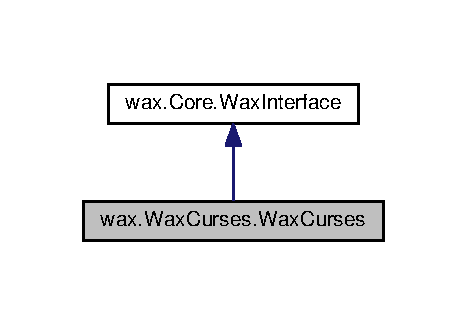
\includegraphics[width=224pt]{classwax_1_1WaxCurses_1_1WaxCurses__inherit__graph}
\end{center}
\end{figure}


Collaboration diagram for wax.\+Wax\+Curses.\+Wax\+Curses\+:
\nopagebreak
\begin{figure}[H]
\begin{center}
\leavevmode
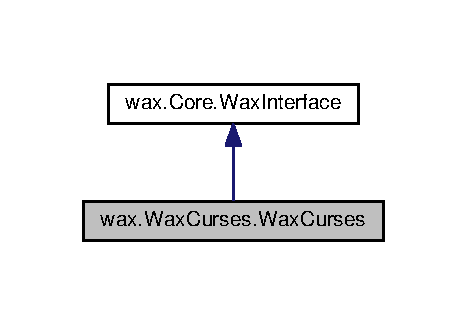
\includegraphics[width=224pt]{classwax_1_1WaxCurses_1_1WaxCurses__coll__graph}
\end{center}
\end{figure}
\subsection*{Public Member Functions}
\begin{DoxyCompactItemize}
\item 
def {\bfseries \+\_\+\+\_\+init\+\_\+\+\_\+} (self)\hypertarget{classwax_1_1WaxCurses_1_1WaxCurses_a8b99fe79c8a55a1ca31a6a3fff6a03a0}{}\label{classwax_1_1WaxCurses_1_1WaxCurses_a8b99fe79c8a55a1ca31a6a3fff6a03a0}

\item 
def {\bfseries start} (s)\hypertarget{classwax_1_1WaxCurses_1_1WaxCurses_adfa97985ee52aa2f691a8672bb716016}{}\label{classwax_1_1WaxCurses_1_1WaxCurses_adfa97985ee52aa2f691a8672bb716016}

\end{DoxyCompactItemize}


\subsection{Detailed Description}
Main class for Wax C\+LI controller After creation, you must bind some actions via \hyperlink{classwax_1_1Core_1_1WaxInterface_af10d87f79dc119f4d5f30cd70ef9feb9}{bind\+\_\+action()} method To start controlling terminal, just call start() 

The documentation for this class was generated from the following file\+:\begin{DoxyCompactItemize}
\item 
wax/Wax\+Curses.\+py\end{DoxyCompactItemize}

\hypertarget{classwax_1_1Core_1_1WaxInterface}{}\section{wax.\+Core.\+Wax\+Interface Class Reference}
\label{classwax_1_1Core_1_1WaxInterface}\index{wax.\+Core.\+Wax\+Interface@{wax.\+Core.\+Wax\+Interface}}


Parent class for Wax\+Curses and Wax\+Server Provides common methods.  


\subsection*{Public Member Functions}
\begin{DoxyCompactItemize}
\item 
def {\bfseries \+\_\+\+\_\+init\+\_\+\+\_\+} (self)\hypertarget{classwax_1_1Core_1_1WaxInterface_a9494be173be6e980524d2e2527583f0b}{}\label{classwax_1_1Core_1_1WaxInterface_a9494be173be6e980524d2e2527583f0b}

\item 
def \hyperlink{classwax_1_1Core_1_1WaxInterface_af10d87f79dc119f4d5f30cd70ef9feb9}{bind\+\_\+action} (self, name, func)
\begin{DoxyCompactList}\small\item\em Bind actions. \end{DoxyCompactList}\item 
def {\bfseries bind\+\_\+key} (self, key, func)\hypertarget{classwax_1_1Core_1_1WaxInterface_a58dd4d72ef0a9123e85ea22f90e48797}{}\label{classwax_1_1Core_1_1WaxInterface_a58dd4d72ef0a9123e85ea22f90e48797}

\end{DoxyCompactItemize}


\subsection{Detailed Description}
Parent class for Wax\+Curses and Wax\+Server Provides common methods. 

\subsection{Member Function Documentation}
\index{wax\+::\+Core\+::\+Wax\+Interface@{wax\+::\+Core\+::\+Wax\+Interface}!bind\+\_\+action@{bind\+\_\+action}}
\index{bind\+\_\+action@{bind\+\_\+action}!wax\+::\+Core\+::\+Wax\+Interface@{wax\+::\+Core\+::\+Wax\+Interface}}
\subsubsection[{\texorpdfstring{bind\+\_\+action(self, name, func)}{bind_action(self, name, func)}}]{\setlength{\rightskip}{0pt plus 5cm}def wax.\+Core.\+Wax\+Interface.\+bind\+\_\+action (
\begin{DoxyParamCaption}
\item[{}]{self, }
\item[{}]{name, }
\item[{}]{func}
\end{DoxyParamCaption}
)}\hypertarget{classwax_1_1Core_1_1WaxInterface_af10d87f79dc119f4d5f30cd70ef9feb9}{}\label{classwax_1_1Core_1_1WaxInterface_af10d87f79dc119f4d5f30cd70ef9feb9}


Bind actions. 


\begin{DoxyParams}{Parameters}
{\em name} & Name of action to trigger it. \\
\hline
{\em func} & A function, that will be called, when action is triggered. That function {\bfseries must accept one parameter}, that is a dictionary with action name and passes variables and it {\bfseries must return \hyperlink{classwax_1_1Core_1_1WForm}{W\+Form} object} to render it. \\
\hline
\end{DoxyParams}


The documentation for this class was generated from the following file\+:\begin{DoxyCompactItemize}
\item 
wax/Core.\+py\end{DoxyCompactItemize}

\hypertarget{classwax_1_1WaxServer_1_1WaxServer}{}\section{wax.\+Wax\+Server.\+Wax\+Server Class Reference}
\label{classwax_1_1WaxServer_1_1WaxServer}\index{wax.\+Wax\+Server.\+Wax\+Server@{wax.\+Wax\+Server.\+Wax\+Server}}


Main class for Wax server You may specify port to start when creating \hyperlink{classwax_1_1WaxServer_1_1WaxServer}{Wax\+Server}.  




Inheritance diagram for wax.\+Wax\+Server.\+Wax\+Server\+:\nopagebreak
\begin{figure}[H]
\begin{center}
\leavevmode
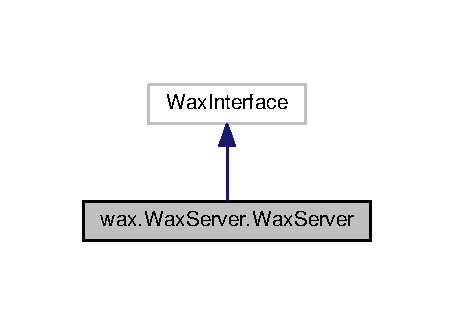
\includegraphics[width=218pt]{classwax_1_1WaxServer_1_1WaxServer__inherit__graph}
\end{center}
\end{figure}


Collaboration diagram for wax.\+Wax\+Server.\+Wax\+Server\+:\nopagebreak
\begin{figure}[H]
\begin{center}
\leavevmode
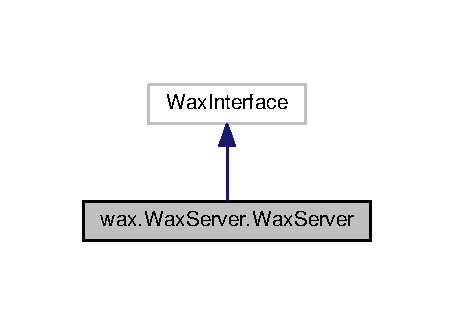
\includegraphics[width=218pt]{classwax_1_1WaxServer_1_1WaxServer__coll__graph}
\end{center}
\end{figure}
\subsection*{Public Member Functions}
\begin{DoxyCompactItemize}
\item 
def \hyperlink{classwax_1_1WaxServer_1_1WaxServer_ac24860098a9231745f96d05a90444187}{\+\_\+\+\_\+init\+\_\+\+\_\+} (self, port=80)
\begin{DoxyCompactList}\small\item\em Constructor. \end{DoxyCompactList}\item 
def \hyperlink{classwax_1_1WaxServer_1_1WaxServer_a95283fc6af92b3c7f28facbd9c7e995f}{start} (self)\hypertarget{classwax_1_1WaxServer_1_1WaxServer_a95283fc6af92b3c7f28facbd9c7e995f}{}\label{classwax_1_1WaxServer_1_1WaxServer_a95283fc6af92b3c7f28facbd9c7e995f}

\begin{DoxyCompactList}\small\item\em Fire it up. \end{DoxyCompactList}\end{DoxyCompactItemize}
\subsection*{Public Attributes}
\begin{DoxyCompactItemize}
\item 
{\bfseries server}\hypertarget{classwax_1_1WaxServer_1_1WaxServer_a2a265dc0e14a20b39c3971395fbadaa1}{}\label{classwax_1_1WaxServer_1_1WaxServer_a2a265dc0e14a20b39c3971395fbadaa1}

\end{DoxyCompactItemize}


\subsection{Detailed Description}
Main class for Wax server You may specify port to start when creating \hyperlink{classwax_1_1WaxServer_1_1WaxServer}{Wax\+Server}. 

After creation, you must bind some actions via bind\+\_\+action() method. To fire it up, just call \hyperlink{classwax_1_1WaxServer_1_1WaxServer_a95283fc6af92b3c7f28facbd9c7e995f}{start()} 

\subsection{Constructor \& Destructor Documentation}
\index{wax\+::\+Wax\+Server\+::\+Wax\+Server@{wax\+::\+Wax\+Server\+::\+Wax\+Server}!\+\_\+\+\_\+init\+\_\+\+\_\+@{\+\_\+\+\_\+init\+\_\+\+\_\+}}
\index{\+\_\+\+\_\+init\+\_\+\+\_\+@{\+\_\+\+\_\+init\+\_\+\+\_\+}!wax\+::\+Wax\+Server\+::\+Wax\+Server@{wax\+::\+Wax\+Server\+::\+Wax\+Server}}
\subsubsection[{\texorpdfstring{\+\_\+\+\_\+init\+\_\+\+\_\+(self, port=80)}{__init__(self, port=80)}}]{\setlength{\rightskip}{0pt plus 5cm}def wax.\+Wax\+Server.\+Wax\+Server.\+\_\+\+\_\+init\+\_\+\+\_\+ (
\begin{DoxyParamCaption}
\item[{}]{self, }
\item[{}]{port = {\ttfamily 80}}
\end{DoxyParamCaption}
)}\hypertarget{classwax_1_1WaxServer_1_1WaxServer_ac24860098a9231745f96d05a90444187}{}\label{classwax_1_1WaxServer_1_1WaxServer_ac24860098a9231745f96d05a90444187}


Constructor. 


\begin{DoxyParams}{Parameters}
{\em port} & Specify port to listen. Default is 80. \\
\hline
\end{DoxyParams}


The documentation for this class was generated from the following file\+:\begin{DoxyCompactItemize}
\item 
wax/Wax\+Server.\+py\end{DoxyCompactItemize}

\hypertarget{classwax_1_1Components_1_1WButton}{}\section{wax.\+Components.\+W\+Button Class Reference}
\label{classwax_1_1Components_1_1WButton}\index{wax.\+Components.\+W\+Button@{wax.\+Components.\+W\+Button}}


Button element.  




Inheritance diagram for wax.\+Components.\+W\+Button\+:
\nopagebreak
\begin{figure}[H]
\begin{center}
\leavevmode
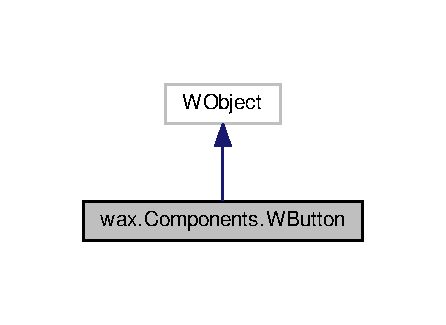
\includegraphics[width=214pt]{classwax_1_1Components_1_1WButton__inherit__graph}
\end{center}
\end{figure}


Collaboration diagram for wax.\+Components.\+W\+Button\+:
\nopagebreak
\begin{figure}[H]
\begin{center}
\leavevmode
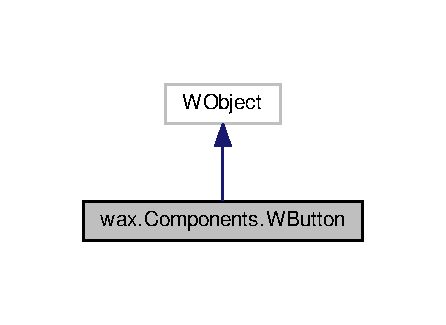
\includegraphics[width=214pt]{classwax_1_1Components_1_1WButton__coll__graph}
\end{center}
\end{figure}
\subsection*{Public Member Functions}
\begin{DoxyCompactItemize}
\item 
def \hyperlink{classwax_1_1Components_1_1WButton_a83f8a36633e5b1bd2450cac551dffc21}{\+\_\+\+\_\+init\+\_\+\+\_\+} (self, text=\char`\"{}Button\char`\"{}, action=\textquotesingle{}\textquotesingle{}, enabled=True, html\+\_\+method\+\_\+post=False)
\begin{DoxyCompactList}\small\item\em Constructor. \end{DoxyCompactList}\item 
def \hyperlink{classwax_1_1Components_1_1WButton_a267e6a05324a1f27470bf05127c462fe}{html} (self)
\begin{DoxyCompactList}\small\item\em Function for rendering H\+T\+ML code of this element. \end{DoxyCompactList}\item 
def {\bfseries render\+\_\+curses} (self, sel=False)\hypertarget{classwax_1_1Components_1_1WButton_abb75f46a3eb9bbeb2a0aa267e4ce0534}{}\label{classwax_1_1Components_1_1WButton_abb75f46a3eb9bbeb2a0aa267e4ce0534}

\end{DoxyCompactItemize}


\subsection{Detailed Description}
Button element. 

\subsection{Constructor \& Destructor Documentation}
\index{wax\+::\+Components\+::\+W\+Button@{wax\+::\+Components\+::\+W\+Button}!\+\_\+\+\_\+init\+\_\+\+\_\+@{\+\_\+\+\_\+init\+\_\+\+\_\+}}
\index{\+\_\+\+\_\+init\+\_\+\+\_\+@{\+\_\+\+\_\+init\+\_\+\+\_\+}!wax\+::\+Components\+::\+W\+Button@{wax\+::\+Components\+::\+W\+Button}}
\subsubsection[{\texorpdfstring{\+\_\+\+\_\+init\+\_\+\+\_\+(self, text=""Button"", action=\textquotesingle{}\textquotesingle{}, enabled=\+True, html\+\_\+method\+\_\+post=\+False)}{__init__(self, text="Button", action='', enabled=True, html_method_post=False)}}]{\setlength{\rightskip}{0pt plus 5cm}def wax.\+Components.\+W\+Button.\+\_\+\+\_\+init\+\_\+\+\_\+ (
\begin{DoxyParamCaption}
\item[{}]{self, }
\item[{}]{text = {\ttfamily \char`\"{}Button\char`\"{}}, }
\item[{}]{action = {\ttfamily \textquotesingle{}\textquotesingle{}}, }
\item[{}]{enabled = {\ttfamily True}, }
\item[{}]{html\+\_\+method\+\_\+post = {\ttfamily False}}
\end{DoxyParamCaption}
)}\hypertarget{classwax_1_1Components_1_1WButton_a83f8a36633e5b1bd2450cac551dffc21}{}\label{classwax_1_1Components_1_1WButton_a83f8a36633e5b1bd2450cac551dffc21}


Constructor. 


\begin{DoxyParams}{Parameters}
{\em text} & Text on the button \\
\hline
{\em enabled} & Is it active to click \\
\hline
{\em visible} & Is it visible on the form \\
\hline
{\em action} & What action it will trigger \\
\hline
\end{DoxyParams}


\subsection{Member Function Documentation}
\index{wax\+::\+Components\+::\+W\+Button@{wax\+::\+Components\+::\+W\+Button}!html@{html}}
\index{html@{html}!wax\+::\+Components\+::\+W\+Button@{wax\+::\+Components\+::\+W\+Button}}
\subsubsection[{\texorpdfstring{html(self)}{html(self)}}]{\setlength{\rightskip}{0pt plus 5cm}def wax.\+Components.\+W\+Button.\+html (
\begin{DoxyParamCaption}
\item[{}]{self}
\end{DoxyParamCaption}
)}\hypertarget{classwax_1_1Components_1_1WButton_a267e6a05324a1f27470bf05127c462fe}{}\label{classwax_1_1Components_1_1WButton_a267e6a05324a1f27470bf05127c462fe}


Function for rendering H\+T\+ML code of this element. 

\begin{DoxyReturn}{Returns}
A string with H\+T\+M\+L-\/code of element 
\end{DoxyReturn}


The documentation for this class was generated from the following file\+:\begin{DoxyCompactItemize}
\item 
wax/Components.\+py\end{DoxyCompactItemize}

\hypertarget{classwax_1_1Components_1_1WCheckBox}{}\section{wax.\+Components.\+W\+Check\+Box Class Reference}
\label{classwax_1_1Components_1_1WCheckBox}\index{wax.\+Components.\+W\+Check\+Box@{wax.\+Components.\+W\+Check\+Box}}


Checkbox element.  




Inheritance diagram for wax.\+Components.\+W\+Check\+Box\+:
\nopagebreak
\begin{figure}[H]
\begin{center}
\leavevmode
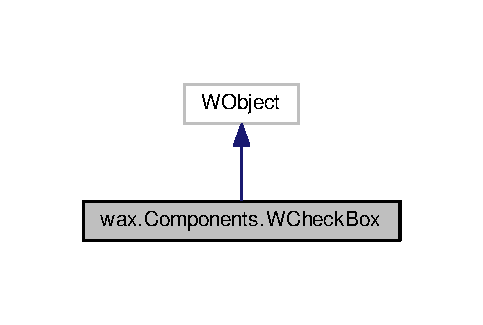
\includegraphics[width=232pt]{classwax_1_1Components_1_1WCheckBox__inherit__graph}
\end{center}
\end{figure}


Collaboration diagram for wax.\+Components.\+W\+Check\+Box\+:
\nopagebreak
\begin{figure}[H]
\begin{center}
\leavevmode
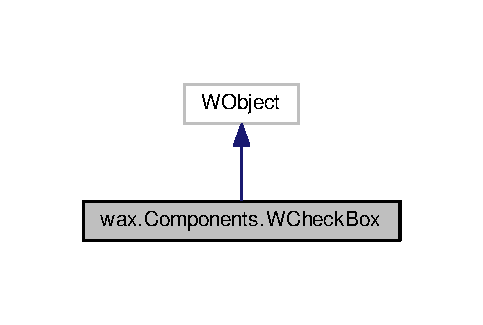
\includegraphics[width=232pt]{classwax_1_1Components_1_1WCheckBox__coll__graph}
\end{center}
\end{figure}
\subsection*{Public Member Functions}
\begin{DoxyCompactItemize}
\item 
def \hyperlink{classwax_1_1Components_1_1WCheckBox_a4be3a9f77c93e57d2feb0755ac3d9ba4}{\+\_\+\+\_\+init\+\_\+\+\_\+} (self, text=\textquotesingle{}Checkbox\textquotesingle{}, name=\textquotesingle{}checkbox\textquotesingle{}, value=False, enabled=True)
\begin{DoxyCompactList}\small\item\em Constructor. \end{DoxyCompactList}\item 
def {\bfseries set\+\_\+value} (self, value)\hypertarget{classwax_1_1Components_1_1WCheckBox_a0b335395de207887683cb755bace5bcc}{}\label{classwax_1_1Components_1_1WCheckBox_a0b335395de207887683cb755bace5bcc}

\item 
def {\bfseries html} (self)\hypertarget{classwax_1_1Components_1_1WCheckBox_a72576669baf815e3573be4afea8118ee}{}\label{classwax_1_1Components_1_1WCheckBox_a72576669baf815e3573be4afea8118ee}

\item 
def {\bfseries render\+\_\+curses} (self, sel=False)\hypertarget{classwax_1_1Components_1_1WCheckBox_a305cdfe963d0ab8c014d67b4b3ec8c2f}{}\label{classwax_1_1Components_1_1WCheckBox_a305cdfe963d0ab8c014d67b4b3ec8c2f}

\end{DoxyCompactItemize}


\subsection{Detailed Description}
Checkbox element. 

\subsection{Constructor \& Destructor Documentation}
\index{wax\+::\+Components\+::\+W\+Check\+Box@{wax\+::\+Components\+::\+W\+Check\+Box}!\+\_\+\+\_\+init\+\_\+\+\_\+@{\+\_\+\+\_\+init\+\_\+\+\_\+}}
\index{\+\_\+\+\_\+init\+\_\+\+\_\+@{\+\_\+\+\_\+init\+\_\+\+\_\+}!wax\+::\+Components\+::\+W\+Check\+Box@{wax\+::\+Components\+::\+W\+Check\+Box}}
\subsubsection[{\texorpdfstring{\+\_\+\+\_\+init\+\_\+\+\_\+(self, text=\textquotesingle{}\+Checkbox\textquotesingle{}, name=\textquotesingle{}checkbox\textquotesingle{}, value=\+False, enabled=\+True)}{__init__(self, text='Checkbox', name='checkbox', value=False, enabled=True)}}]{\setlength{\rightskip}{0pt plus 5cm}def wax.\+Components.\+W\+Check\+Box.\+\_\+\+\_\+init\+\_\+\+\_\+ (
\begin{DoxyParamCaption}
\item[{}]{self, }
\item[{}]{text = {\ttfamily \textquotesingle{}Checkbox\textquotesingle{}}, }
\item[{}]{name = {\ttfamily \textquotesingle{}checkbox\textquotesingle{}}, }
\item[{}]{value = {\ttfamily False}, }
\item[{}]{enabled = {\ttfamily True}}
\end{DoxyParamCaption}
)}\hypertarget{classwax_1_1Components_1_1WCheckBox_a4be3a9f77c93e57d2feb0755ac3d9ba4}{}\label{classwax_1_1Components_1_1WCheckBox_a4be3a9f77c93e57d2feb0755ac3d9ba4}


Constructor. 


\begin{DoxyParams}{Parameters}
{\em text} & Text on checkbox \\
\hline
{\em value} & Boolean value, is checkbox checked or not \\
\hline
{\em enabled} & Is value can be changed \\
\hline
{\em name} & name to be passed to args\mbox{[}\mbox{]} \\
\hline
\end{DoxyParams}


The documentation for this class was generated from the following file\+:\begin{DoxyCompactItemize}
\item 
wax/Components.\+py\end{DoxyCompactItemize}

\hypertarget{classwax_1_1Core_1_1WForm}{}\section{wax.\+Core.\+W\+Form Class Reference}
\label{classwax_1_1Core_1_1WForm}\index{wax.\+Core.\+W\+Form@{wax.\+Core.\+W\+Form}}


Form class Form is a basic class to render form on the Web-\/page or in the terminal.  


\subsection*{Public Member Functions}
\begin{DoxyCompactItemize}
\item 
def \hyperlink{classwax_1_1Core_1_1WForm_ae21d181e9ad6153bceda8265a6e9ce8c}{\+\_\+\+\_\+init\+\_\+\+\_\+} (self, title=\char`\"{}Wax Form\char`\"{})
\begin{DoxyCompactList}\small\item\em Constructor. \end{DoxyCompactList}\item 
def \hyperlink{classwax_1_1Core_1_1WForm_a9d093d9e1309adf5b8be93add1b8a692}{set\+\_\+title} (self, title)\hypertarget{classwax_1_1Core_1_1WForm_a9d093d9e1309adf5b8be93add1b8a692}{}\label{classwax_1_1Core_1_1WForm_a9d093d9e1309adf5b8be93add1b8a692}

\begin{DoxyCompactList}\small\item\em Change title title New title. \end{DoxyCompactList}\item 
def \hyperlink{classwax_1_1Core_1_1WForm_ade1b1967b65f7f5a91a64ea6e82314cd}{html} (self)\hypertarget{classwax_1_1Core_1_1WForm_ade1b1967b65f7f5a91a64ea6e82314cd}{}\label{classwax_1_1Core_1_1WForm_ade1b1967b65f7f5a91a64ea6e82314cd}

\begin{DoxyCompactList}\small\item\em This function returns html-\/formatted form. \end{DoxyCompactList}\item 
def \hyperlink{classwax_1_1Core_1_1WForm_ad63eb68566b51859cd2271be2c73e1ad}{add\+\_\+object} (self, obj)
\begin{DoxyCompactList}\small\item\em Add a component to this form. \end{DoxyCompactList}\end{DoxyCompactItemize}


\subsection{Detailed Description}
Form class Form is a basic class to render form on the Web-\/page or in the terminal. 

It must be returned from action functions. 

\subsection{Constructor \& Destructor Documentation}
\index{wax\+::\+Core\+::\+W\+Form@{wax\+::\+Core\+::\+W\+Form}!\+\_\+\+\_\+init\+\_\+\+\_\+@{\+\_\+\+\_\+init\+\_\+\+\_\+}}
\index{\+\_\+\+\_\+init\+\_\+\+\_\+@{\+\_\+\+\_\+init\+\_\+\+\_\+}!wax\+::\+Core\+::\+W\+Form@{wax\+::\+Core\+::\+W\+Form}}
\subsubsection[{\texorpdfstring{\+\_\+\+\_\+init\+\_\+\+\_\+(self, title=""Wax Form"")}{__init__(self, title="Wax Form")}}]{\setlength{\rightskip}{0pt plus 5cm}def wax.\+Core.\+W\+Form.\+\_\+\+\_\+init\+\_\+\+\_\+ (
\begin{DoxyParamCaption}
\item[{}]{self, }
\item[{}]{title = {\ttfamily \char`\"{}Wax~Form\char`\"{}}}
\end{DoxyParamCaption}
)}\hypertarget{classwax_1_1Core_1_1WForm_ae21d181e9ad6153bceda8265a6e9ce8c}{}\label{classwax_1_1Core_1_1WForm_ae21d181e9ad6153bceda8265a6e9ce8c}


Constructor. 


\begin{DoxyParams}{Parameters}
{\em title} & Title of form. \\
\hline
\end{DoxyParams}


\subsection{Member Function Documentation}
\index{wax\+::\+Core\+::\+W\+Form@{wax\+::\+Core\+::\+W\+Form}!add\+\_\+object@{add\+\_\+object}}
\index{add\+\_\+object@{add\+\_\+object}!wax\+::\+Core\+::\+W\+Form@{wax\+::\+Core\+::\+W\+Form}}
\subsubsection[{\texorpdfstring{add\+\_\+object(self, obj)}{add_object(self, obj)}}]{\setlength{\rightskip}{0pt plus 5cm}def wax.\+Core.\+W\+Form.\+add\+\_\+object (
\begin{DoxyParamCaption}
\item[{}]{self, }
\item[{}]{obj}
\end{DoxyParamCaption}
)}\hypertarget{classwax_1_1Core_1_1WForm_ad63eb68566b51859cd2271be2c73e1ad}{}\label{classwax_1_1Core_1_1WForm_ad63eb68566b51859cd2271be2c73e1ad}


Add a component to this form. 


\begin{DoxyParams}{Parameters}
{\em obj} & \hyperlink{classwax_1_1Core_1_1WObject}{W\+Object} to add \\
\hline
\end{DoxyParams}
\begin{DoxyReturn}{Returns}
Pointer to this component
\end{DoxyReturn}
Type\+Error if obj isn\textquotesingle{}t \hyperlink{classwax_1_1Core_1_1WObject}{W\+Object} 

The documentation for this class was generated from the following file\+:\begin{DoxyCompactItemize}
\item 
wax/Core.\+py\end{DoxyCompactItemize}

\hypertarget{classwax_1_1Components_1_1WFormsCarousel}{}\section{wax.\+Components.\+W\+Forms\+Carousel Class Reference}
\label{classwax_1_1Components_1_1WFormsCarousel}\index{wax.\+Components.\+W\+Forms\+Carousel@{wax.\+Components.\+W\+Forms\+Carousel}}


Forms carousel to navigate between forms.  




Inheritance diagram for wax.\+Components.\+W\+Forms\+Carousel\+:\nopagebreak
\begin{figure}[H]
\begin{center}
\leavevmode
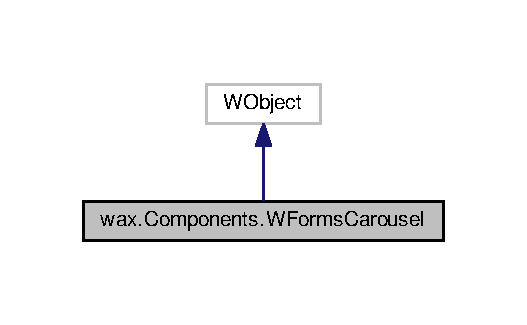
\includegraphics[width=253pt]{classwax_1_1Components_1_1WFormsCarousel__inherit__graph}
\end{center}
\end{figure}


Collaboration diagram for wax.\+Components.\+W\+Forms\+Carousel\+:\nopagebreak
\begin{figure}[H]
\begin{center}
\leavevmode
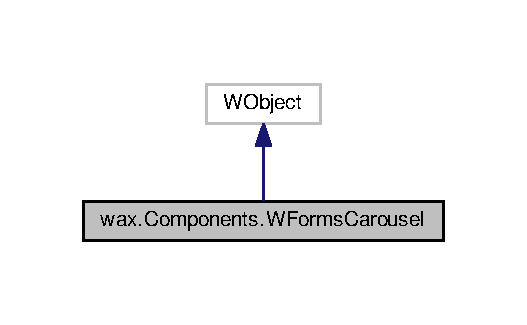
\includegraphics[width=253pt]{classwax_1_1Components_1_1WFormsCarousel__coll__graph}
\end{center}
\end{figure}
\subsection*{Public Member Functions}
\begin{DoxyCompactItemize}
\item 
def \hyperlink{classwax_1_1Components_1_1WFormsCarousel_a853fcd7ebd11dfb818ecabdf043b15e9}{\+\_\+\+\_\+init\+\_\+\+\_\+} (self, tabs=\mbox{[}$\,$\mbox{]}, current\+\_\+action=None, enabled=True, width=50)
\begin{DoxyCompactList}\small\item\em Constructor. \end{DoxyCompactList}\item 
def {\bfseries html} (self)\hypertarget{classwax_1_1Components_1_1WFormsCarousel_a3d759bcebb338b88ce0d2c92a2c863b7}{}\label{classwax_1_1Components_1_1WFormsCarousel_a3d759bcebb338b88ce0d2c92a2c863b7}

\item 
def {\bfseries render\+\_\+curses} (self, sel=False)\hypertarget{classwax_1_1Components_1_1WFormsCarousel_a2a4d988d443a2e556e8023c9daeb7959}{}\label{classwax_1_1Components_1_1WFormsCarousel_a2a4d988d443a2e556e8023c9daeb7959}

\end{DoxyCompactItemize}


\subsection{Detailed Description}
Forms carousel to navigate between forms. 

\subsection{Constructor \& Destructor Documentation}
\index{wax\+::\+Components\+::\+W\+Forms\+Carousel@{wax\+::\+Components\+::\+W\+Forms\+Carousel}!\+\_\+\+\_\+init\+\_\+\+\_\+@{\+\_\+\+\_\+init\+\_\+\+\_\+}}
\index{\+\_\+\+\_\+init\+\_\+\+\_\+@{\+\_\+\+\_\+init\+\_\+\+\_\+}!wax\+::\+Components\+::\+W\+Forms\+Carousel@{wax\+::\+Components\+::\+W\+Forms\+Carousel}}
\subsubsection[{\texorpdfstring{\+\_\+\+\_\+init\+\_\+\+\_\+(self, tabs=[], current\+\_\+action=\+None, enabled=\+True, width=50)}{__init__(self, tabs=[], current_action=None, enabled=True, width=50)}}]{\setlength{\rightskip}{0pt plus 5cm}def wax.\+Components.\+W\+Forms\+Carousel.\+\_\+\+\_\+init\+\_\+\+\_\+ (
\begin{DoxyParamCaption}
\item[{}]{self, }
\item[{}]{tabs = {\ttfamily \mbox{[}\mbox{]}}, }
\item[{}]{current\+\_\+action = {\ttfamily None}, }
\item[{}]{enabled = {\ttfamily True}, }
\item[{}]{width = {\ttfamily 50}}
\end{DoxyParamCaption}
)}\hypertarget{classwax_1_1Components_1_1WFormsCarousel_a853fcd7ebd11dfb818ecabdf043b15e9}{}\label{classwax_1_1Components_1_1WFormsCarousel_a853fcd7ebd11dfb818ecabdf043b15e9}


Constructor. 


\begin{DoxyParams}{Parameters}
{\em tabs} & List of tuples of actions and it\textquotesingle{}s labels \\
\hline
{\em current\+\_\+action} & Current action name, needed for correct working. Pass args\mbox{[}\textquotesingle{}action\textquotesingle{}\mbox{]} to it. \\
\hline
{\em enabled} & is carousel enabled \\
\hline
{\em width} & width of carousel in terminal mode(in symbols) \\
\hline
\end{DoxyParams}


The documentation for this class was generated from the following file\+:\begin{DoxyCompactItemize}
\item 
wax/Components.\+py\end{DoxyCompactItemize}

\hypertarget{classwax_1_1Components_1_1WLabel}{}\section{wax.\+Components.\+W\+Label Class Reference}
\label{classwax_1_1Components_1_1WLabel}\index{wax.\+Components.\+W\+Label@{wax.\+Components.\+W\+Label}}


Label element.  




Inheritance diagram for wax.\+Components.\+W\+Label\+:\nopagebreak
\begin{figure}[H]
\begin{center}
\leavevmode
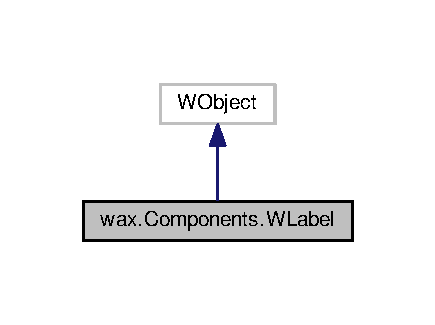
\includegraphics[width=209pt]{classwax_1_1Components_1_1WLabel__inherit__graph}
\end{center}
\end{figure}


Collaboration diagram for wax.\+Components.\+W\+Label\+:\nopagebreak
\begin{figure}[H]
\begin{center}
\leavevmode
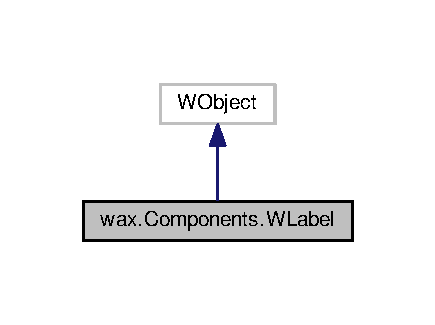
\includegraphics[width=209pt]{classwax_1_1Components_1_1WLabel__coll__graph}
\end{center}
\end{figure}
\subsection*{Public Member Functions}
\begin{DoxyCompactItemize}
\item 
def \hyperlink{classwax_1_1Components_1_1WLabel_a36220e24b690fec62b8c8c38a0c8d9c3}{\+\_\+\+\_\+init\+\_\+\+\_\+} (self, text=\char`\"{}Label\char`\"{})
\begin{DoxyCompactList}\small\item\em Constructor. \end{DoxyCompactList}\item 
def {\bfseries set\+\_\+value} (self, value)\hypertarget{classwax_1_1Components_1_1WLabel_a171e82f31486f1e5d25fce5d6368b04b}{}\label{classwax_1_1Components_1_1WLabel_a171e82f31486f1e5d25fce5d6368b04b}

\item 
def \hyperlink{classwax_1_1Components_1_1WLabel_a674a083f20dad3bae26a691b2e020028}{set\+\_\+style} (self, bold=False, italic=False)
\begin{DoxyCompactList}\small\item\em Setting font style. \end{DoxyCompactList}\item 
def \hyperlink{classwax_1_1Components_1_1WLabel_a61037e48c8f371f7270702258890e918}{html} (self)
\begin{DoxyCompactList}\small\item\em Function for rendering H\+T\+ML code of this element. \end{DoxyCompactList}\item 
def {\bfseries render\+\_\+curses} (self, sel=False)\hypertarget{classwax_1_1Components_1_1WLabel_a5f468ed72b4f54f02ea981a4e2a72536}{}\label{classwax_1_1Components_1_1WLabel_a5f468ed72b4f54f02ea981a4e2a72536}

\end{DoxyCompactItemize}


\subsection{Detailed Description}
Label element. 

\subsection{Constructor \& Destructor Documentation}
\index{wax\+::\+Components\+::\+W\+Label@{wax\+::\+Components\+::\+W\+Label}!\+\_\+\+\_\+init\+\_\+\+\_\+@{\+\_\+\+\_\+init\+\_\+\+\_\+}}
\index{\+\_\+\+\_\+init\+\_\+\+\_\+@{\+\_\+\+\_\+init\+\_\+\+\_\+}!wax\+::\+Components\+::\+W\+Label@{wax\+::\+Components\+::\+W\+Label}}
\subsubsection[{\texorpdfstring{\+\_\+\+\_\+init\+\_\+\+\_\+(self, text=""Label"")}{__init__(self, text="Label")}}]{\setlength{\rightskip}{0pt plus 5cm}def wax.\+Components.\+W\+Label.\+\_\+\+\_\+init\+\_\+\+\_\+ (
\begin{DoxyParamCaption}
\item[{}]{self, }
\item[{}]{text = {\ttfamily \char`\"{}Label\char`\"{}}}
\end{DoxyParamCaption}
)}\hypertarget{classwax_1_1Components_1_1WLabel_a36220e24b690fec62b8c8c38a0c8d9c3}{}\label{classwax_1_1Components_1_1WLabel_a36220e24b690fec62b8c8c38a0c8d9c3}


Constructor. 


\begin{DoxyParams}{Parameters}
{\em text} & Text to be shown in element \\
\hline
\end{DoxyParams}


\subsection{Member Function Documentation}
\index{wax\+::\+Components\+::\+W\+Label@{wax\+::\+Components\+::\+W\+Label}!html@{html}}
\index{html@{html}!wax\+::\+Components\+::\+W\+Label@{wax\+::\+Components\+::\+W\+Label}}
\subsubsection[{\texorpdfstring{html(self)}{html(self)}}]{\setlength{\rightskip}{0pt plus 5cm}def wax.\+Components.\+W\+Label.\+html (
\begin{DoxyParamCaption}
\item[{}]{self}
\end{DoxyParamCaption}
)}\hypertarget{classwax_1_1Components_1_1WLabel_a61037e48c8f371f7270702258890e918}{}\label{classwax_1_1Components_1_1WLabel_a61037e48c8f371f7270702258890e918}


Function for rendering H\+T\+ML code of this element. 

\begin{DoxyReturn}{Returns}
A string with H\+T\+M\+L-\/code of element 
\end{DoxyReturn}
\index{wax\+::\+Components\+::\+W\+Label@{wax\+::\+Components\+::\+W\+Label}!set\+\_\+style@{set\+\_\+style}}
\index{set\+\_\+style@{set\+\_\+style}!wax\+::\+Components\+::\+W\+Label@{wax\+::\+Components\+::\+W\+Label}}
\subsubsection[{\texorpdfstring{set\+\_\+style(self, bold=\+False, italic=\+False)}{set_style(self, bold=False, italic=False)}}]{\setlength{\rightskip}{0pt plus 5cm}def wax.\+Components.\+W\+Label.\+set\+\_\+style (
\begin{DoxyParamCaption}
\item[{}]{self, }
\item[{}]{bold = {\ttfamily False}, }
\item[{}]{italic = {\ttfamily False}}
\end{DoxyParamCaption}
)}\hypertarget{classwax_1_1Components_1_1WLabel_a674a083f20dad3bae26a691b2e020028}{}\label{classwax_1_1Components_1_1WLabel_a674a083f20dad3bae26a691b2e020028}


Setting font style. 


\begin{DoxyParams}{Parameters}
{\em bold} & Bold font \\
\hline
{\em italic} & Italic font \\
\hline
\end{DoxyParams}


The documentation for this class was generated from the following file\+:\begin{DoxyCompactItemize}
\item 
wax/Components.\+py\end{DoxyCompactItemize}

\hypertarget{classwax_1_1Core_1_1WObject}{}\section{wax.\+Core.\+W\+Object Class Reference}
\label{classwax_1_1Core_1_1WObject}\index{wax.\+Core.\+W\+Object@{wax.\+Core.\+W\+Object}}


Parent class for all G\+UI elements, such as Label, Text\+Edit or Button.  


\subsection*{Public Member Functions}
\begin{DoxyCompactItemize}
\item 
def \hyperlink{classwax_1_1Core_1_1WObject_ae6a315f847d25f16d9238af0a52adbdd}{\+\_\+\+\_\+init\+\_\+\+\_\+} (self, enabled=True)
\begin{DoxyCompactList}\small\item\em Constructor. \end{DoxyCompactList}\item 
def {\bfseries set\+\_\+value} (self, value)\hypertarget{classwax_1_1Core_1_1WObject_a92e17df52d239fb808a7dc35b993111b}{}\label{classwax_1_1Core_1_1WObject_a92e17df52d239fb808a7dc35b993111b}

\item 
def \hyperlink{classwax_1_1Core_1_1WObject_a41c9d6f3ac6431512b954df3afe8b521}{html} (self)
\begin{DoxyCompactList}\small\item\em Function for rendering H\+T\+ML code of this element. \end{DoxyCompactList}\item 
def \hyperlink{classwax_1_1Core_1_1WObject_a6b02871acf93de9352856b6f543dd4b1}{render\+\_\+curses} (self, sel=False)
\begin{DoxyCompactList}\small\item\em Render this object to a curses screen. \end{DoxyCompactList}\item 
def \hyperlink{classwax_1_1Core_1_1WObject_ac127564b44b2495ee987a4f6a61f01e1}{set\+\_\+enabled} (self, state)
\begin{DoxyCompactList}\small\item\em Setting active state of element. \end{DoxyCompactList}\end{DoxyCompactItemize}


\subsection{Detailed Description}
Parent class for all G\+UI elements, such as Label, Text\+Edit or Button. 

\subsection{Constructor \& Destructor Documentation}
\index{wax\+::\+Core\+::\+W\+Object@{wax\+::\+Core\+::\+W\+Object}!\+\_\+\+\_\+init\+\_\+\+\_\+@{\+\_\+\+\_\+init\+\_\+\+\_\+}}
\index{\+\_\+\+\_\+init\+\_\+\+\_\+@{\+\_\+\+\_\+init\+\_\+\+\_\+}!wax\+::\+Core\+::\+W\+Object@{wax\+::\+Core\+::\+W\+Object}}
\subsubsection[{\texorpdfstring{\+\_\+\+\_\+init\+\_\+\+\_\+(self, enabled=\+True)}{__init__(self, enabled=True)}}]{\setlength{\rightskip}{0pt plus 5cm}def wax.\+Core.\+W\+Object.\+\_\+\+\_\+init\+\_\+\+\_\+ (
\begin{DoxyParamCaption}
\item[{}]{self, }
\item[{}]{enabled = {\ttfamily True}}
\end{DoxyParamCaption}
)}\hypertarget{classwax_1_1Core_1_1WObject_ae6a315f847d25f16d9238af0a52adbdd}{}\label{classwax_1_1Core_1_1WObject_ae6a315f847d25f16d9238af0a52adbdd}


Constructor. 


\begin{DoxyParams}{Parameters}
{\em visible} & Is element must be shown on the form \\
\hline
{\em enabled} & Is element able to change it\textquotesingle{}s value or grayed \\
\hline
\end{DoxyParams}


\subsection{Member Function Documentation}
\index{wax\+::\+Core\+::\+W\+Object@{wax\+::\+Core\+::\+W\+Object}!html@{html}}
\index{html@{html}!wax\+::\+Core\+::\+W\+Object@{wax\+::\+Core\+::\+W\+Object}}
\subsubsection[{\texorpdfstring{html(self)}{html(self)}}]{\setlength{\rightskip}{0pt plus 5cm}def wax.\+Core.\+W\+Object.\+html (
\begin{DoxyParamCaption}
\item[{}]{self}
\end{DoxyParamCaption}
)}\hypertarget{classwax_1_1Core_1_1WObject_a41c9d6f3ac6431512b954df3afe8b521}{}\label{classwax_1_1Core_1_1WObject_a41c9d6f3ac6431512b954df3afe8b521}


Function for rendering H\+T\+ML code of this element. 

\begin{DoxyReturn}{Returns}
A string with H\+T\+M\+L-\/code of element 
\end{DoxyReturn}
\index{wax\+::\+Core\+::\+W\+Object@{wax\+::\+Core\+::\+W\+Object}!render\+\_\+curses@{render\+\_\+curses}}
\index{render\+\_\+curses@{render\+\_\+curses}!wax\+::\+Core\+::\+W\+Object@{wax\+::\+Core\+::\+W\+Object}}
\subsubsection[{\texorpdfstring{render\+\_\+curses(self, sel=\+False)}{render_curses(self, sel=False)}}]{\setlength{\rightskip}{0pt plus 5cm}def wax.\+Core.\+W\+Object.\+render\+\_\+curses (
\begin{DoxyParamCaption}
\item[{}]{self, }
\item[{}]{sel = {\ttfamily False}}
\end{DoxyParamCaption}
)}\hypertarget{classwax_1_1Core_1_1WObject_a6b02871acf93de9352856b6f543dd4b1}{}\label{classwax_1_1Core_1_1WObject_a6b02871acf93de9352856b6f543dd4b1}


Render this object to a curses screen. 


\begin{DoxyParams}{Parameters}
{\em y} & Y-\/coord on the screen \\
\hline
{\em x} & X-\/coord on the screen \\
\hline
{\em scr} & curses screen to render\\
\hline
{\em sel} & component must be rendered as selected \\
\hline
\end{DoxyParams}
\index{wax\+::\+Core\+::\+W\+Object@{wax\+::\+Core\+::\+W\+Object}!set\+\_\+enabled@{set\+\_\+enabled}}
\index{set\+\_\+enabled@{set\+\_\+enabled}!wax\+::\+Core\+::\+W\+Object@{wax\+::\+Core\+::\+W\+Object}}
\subsubsection[{\texorpdfstring{set\+\_\+enabled(self, state)}{set_enabled(self, state)}}]{\setlength{\rightskip}{0pt plus 5cm}def wax.\+Core.\+W\+Object.\+set\+\_\+enabled (
\begin{DoxyParamCaption}
\item[{}]{self, }
\item[{}]{state}
\end{DoxyParamCaption}
)}\hypertarget{classwax_1_1Core_1_1WObject_ac127564b44b2495ee987a4f6a61f01e1}{}\label{classwax_1_1Core_1_1WObject_ac127564b44b2495ee987a4f6a61f01e1}


Setting active state of element. 

If element is inactive, it grayed and unable to change value.


\begin{DoxyParams}{Parameters}
{\em state} & Enabled state of element. Must be value of True or False. True for active and False for inactive \\
\hline
\end{DoxyParams}


The documentation for this class was generated from the following file\+:\begin{DoxyCompactItemize}
\item 
wax/Core.\+py\end{DoxyCompactItemize}

\hypertarget{classwax_1_1Components_1_1WTextEdit}{}\section{wax.\+Components.\+W\+Text\+Edit Class Reference}
\label{classwax_1_1Components_1_1WTextEdit}\index{wax.\+Components.\+W\+Text\+Edit@{wax.\+Components.\+W\+Text\+Edit}}


Text\+Edit element.  




Inheritance diagram for wax.\+Components.\+W\+Text\+Edit\+:\nopagebreak
\begin{figure}[H]
\begin{center}
\leavevmode
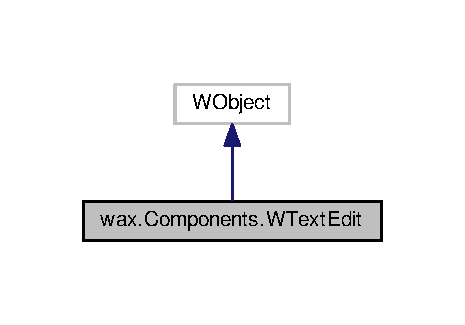
\includegraphics[width=223pt]{classwax_1_1Components_1_1WTextEdit__inherit__graph}
\end{center}
\end{figure}


Collaboration diagram for wax.\+Components.\+W\+Text\+Edit\+:\nopagebreak
\begin{figure}[H]
\begin{center}
\leavevmode
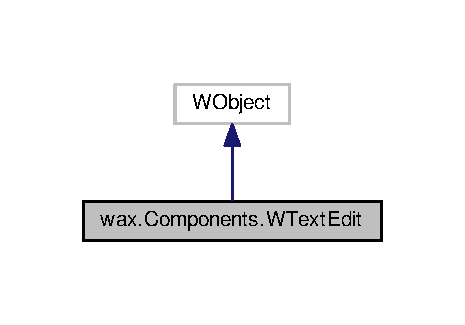
\includegraphics[width=223pt]{classwax_1_1Components_1_1WTextEdit__coll__graph}
\end{center}
\end{figure}
\subsection*{Public Member Functions}
\begin{DoxyCompactItemize}
\item 
def \hyperlink{classwax_1_1Components_1_1WTextEdit_a447086ab6d370b7b345ee5d7d9d1ef45}{\+\_\+\+\_\+init\+\_\+\+\_\+} (self, label=\char`\"{}Edit\char`\"{}, value=\char`\"{}\char`\"{}, size=40, password=False, enabled=True, name=\char`\"{}edit\char`\"{})
\begin{DoxyCompactList}\small\item\em Constructor. \end{DoxyCompactList}\item 
def \hyperlink{classwax_1_1Components_1_1WTextEdit_a38ad3f43e8d97547f250930be64603f6}{html} (self)
\begin{DoxyCompactList}\small\item\em Function for rendering H\+T\+ML code of this element. \end{DoxyCompactList}\item 
def {\bfseries render\+\_\+curses} (self, sel=False)\hypertarget{classwax_1_1Components_1_1WTextEdit_a70d9ca04df9a601a1e4cc8ac83beed85}{}\label{classwax_1_1Components_1_1WTextEdit_a70d9ca04df9a601a1e4cc8ac83beed85}

\end{DoxyCompactItemize}


\subsection{Detailed Description}
Text\+Edit element. 

\subsection{Constructor \& Destructor Documentation}
\index{wax\+::\+Components\+::\+W\+Text\+Edit@{wax\+::\+Components\+::\+W\+Text\+Edit}!\+\_\+\+\_\+init\+\_\+\+\_\+@{\+\_\+\+\_\+init\+\_\+\+\_\+}}
\index{\+\_\+\+\_\+init\+\_\+\+\_\+@{\+\_\+\+\_\+init\+\_\+\+\_\+}!wax\+::\+Components\+::\+W\+Text\+Edit@{wax\+::\+Components\+::\+W\+Text\+Edit}}
\subsubsection[{\texorpdfstring{\+\_\+\+\_\+init\+\_\+\+\_\+(self, label=""Edit"", value="""", size=40, password=\+False, enabled=\+True, name=""edit"")}{__init__(self, label="Edit", value="", size=40, password=False, enabled=True, name="edit")}}]{\setlength{\rightskip}{0pt plus 5cm}def wax.\+Components.\+W\+Text\+Edit.\+\_\+\+\_\+init\+\_\+\+\_\+ (
\begin{DoxyParamCaption}
\item[{}]{self, }
\item[{}]{label = {\ttfamily \char`\"{}Edit\char`\"{}}, }
\item[{}]{value = {\ttfamily \char`\"{}\char`\"{}}, }
\item[{}]{size = {\ttfamily 40}, }
\item[{}]{password = {\ttfamily False}, }
\item[{}]{enabled = {\ttfamily True}, }
\item[{}]{name = {\ttfamily \char`\"{}edit\char`\"{}}}
\end{DoxyParamCaption}
)}\hypertarget{classwax_1_1Components_1_1WTextEdit_a447086ab6d370b7b345ee5d7d9d1ef45}{}\label{classwax_1_1Components_1_1WTextEdit_a447086ab6d370b7b345ee5d7d9d1ef45}


Constructor. 


\begin{DoxyParams}{Parameters}
{\em label} & Text before edit bot \\
\hline
{\em value} & Initial value entered in the box \\
\hline
{\em size} & Size of box \\
\hline
{\em password} & Is value hidden above asterisks \\
\hline
{\em name} & Name of field in variables dict to store its value \\
\hline
{\em enabled} & Is it active to change its value \\
\hline
\end{DoxyParams}


\subsection{Member Function Documentation}
\index{wax\+::\+Components\+::\+W\+Text\+Edit@{wax\+::\+Components\+::\+W\+Text\+Edit}!html@{html}}
\index{html@{html}!wax\+::\+Components\+::\+W\+Text\+Edit@{wax\+::\+Components\+::\+W\+Text\+Edit}}
\subsubsection[{\texorpdfstring{html(self)}{html(self)}}]{\setlength{\rightskip}{0pt plus 5cm}def wax.\+Components.\+W\+Text\+Edit.\+html (
\begin{DoxyParamCaption}
\item[{}]{self}
\end{DoxyParamCaption}
)}\hypertarget{classwax_1_1Components_1_1WTextEdit_a38ad3f43e8d97547f250930be64603f6}{}\label{classwax_1_1Components_1_1WTextEdit_a38ad3f43e8d97547f250930be64603f6}


Function for rendering H\+T\+ML code of this element. 

\begin{DoxyReturn}{Returns}
A string with H\+T\+M\+L-\/code of element 
\end{DoxyReturn}


The documentation for this class was generated from the following file\+:\begin{DoxyCompactItemize}
\item 
wax/Components.\+py\end{DoxyCompactItemize}

%--- End generated contents ---

% Index
\backmatter
\newpage
\phantomsection
\clearemptydoublepage
\addcontentsline{toc}{chapter}{Index}
\printindex

\end{document}
